\section{Einleitung}

\subsection{Motivation und Problemstellung}
In der heutigen Zeit erweist sich Flexibilität als eine immer bedeutendere Determinante für den Erfolg von Unternehmen. Demnach müssen diese stets in der Lage sein, sich effizient an verändernde Marktbedingungen anzupassen. Ein Konzept, um diese schnellen Innovationszyklen zu realisieren, stellt die \textit{Composable-Enterprise-Architektur (CEA)} dar. In einer CEA werden isolierte Software-Komponenten zu einem homogenen Gesamtsystem integriert \cite{.20230313}. Martin Henning Head of New Ventures and Technologies bei der SAP, bemerkt, dass Unternehmen mit diesem Architekturkonzept nicht länger auf \enquote{rigide Systeme} angewiesen sind, sondern vielmehr in der Lage sind Geschäftsprozesse auf Grundlage modularer Bausteinen zusammenzusetzen \cite{Galer.20221019}. Dieser Trend scheint nicht nur bei der SAP, sondern ebenfalls bei anderen Unternehmen angekommen zu sein. So wurde in Gartners Top-Trend-Forschung 2022 prognostiziert, dass bis zum Jahr 2024 80 Prozent der befragten Chief Information Officers (\acs{CIO}s) die modulare Gestaltung von Geschäftsprozessen als eine der fünf wichtigsten Gründe für betriebliches Wachstum betrachten werden \cite{Gartner.20230408}. Um die Geschäftsprozesse in einer CEA noch individueller auf die eigenen Bedürfnisse zuschneiden zu können, neigen Unternehmen dazu, die bestehende Architektur um eigenentwickelte modulare Bausteine zu erweitern. Damit Effizienz und Anpassungsfähigkeit vollständig ausgeschöpft werden kann, ist es unerlässlich, dass diese Bausteine schnell bereitgestellt und in das bestehende System integriert werden. Diese  Softwarebereitstellungsprozesse sollten dabei weitestgehend automatisiert werden. Somit können Fehler frühzeitig erkannt und Software mit höherer Zuverlässigkeit in die Produktivsysteme der Anwender integrieren werden. Zudem kann in zyklischen Überprüfungen sichergestellt werden, dass die Geschäftsanforderungen aller Stakeholder stets erfüllt sind und somit eine qualitativ hochwertige Code-Basis zur Verfügung gestellt wird \cite[471]{Zampetti.92720211012021}. Im Vergleich zum traditionellen Anwendungsdesign benötigt es in einer CEA jedoch agilere und flexiblere Bereitstellungsprozesse, um eine hohe Interoperabilität der einzelnen Bausteine gewährleisten.




\subsection{Zielsetzung und Abgrenzung}
Die technische Beratungsabteilung SAP Data Technology Service (\acs{SAP DTS}) unterstützt Kunden bei der Implementierung einer CEA auf der SAP-Cloud-Plattform. 
Ein essenzielles Thema stellt in diesem Kontext ebenfalls eine Beratungsleistung bezüglich der Implementierung von Software-Bereitstellungsprozessen dar. Um diese Vorgänge zu automatisieren, werden von der SAP i.d.R. drei verschiedene Tools vorgeschlagen. Dazu gehört Azure Pipelines, Jenkins und SAP Continuous Integration and Delivery (\acs{SAP CI/CD}). Ziel der Arbeit ist deshalb, zu evaluieren, welches dieser Tools am besten zur Bereitstellung von Cloud-Software für CEA geeignet ist. Darüber hinaus soll eine ganzheitliche Bereitstellungsstrategie für Composable Enterprises (\acs{CE}s) entwickelt werden. Mit dieser wird dargelegt, wie CEs diese Tools einsetzen können, um ihre Bereitstellungsprozesse zu optimieren.\\ Daraus resultiert folgende Forschungsfrage:\\
\textit{Welches Tool bietet zur Automatisierung der Bereitstellungsprozesse für Composable-\-Enterprise-Architekturen den größten Mehrwert?}\\
Im Rahmen der Zielsetzung werden die folgenden Abgrenzungen vorgenommen: Die Evaluation umfasst ausschließlich die Bereitstellung von Software in der Cloud-Foundry-Laufzeitumgebung der SAP-Cloud-Plattform. Zudem beschränkt sich die Analyse der Bereitstellungs-Tools auf Anwendungen welche, mit SAP CAP Node sowie SAP UI5 entwickelt wurden. Diese Abgrenzung wird gezogen, da das SAP DTS ausschließlich in diesen Technologien berät.  

\subsection{Aufbau der Arbeit}
Die theoretischen Grundlagen beginnen mit der Begriffsdefinition und Abgrenzung der CEA. Im Anschluss werden technologische Konzepte der CEA erläutert. Dabei wird dargelegt, wie CEs ihre Architektur gestalten müssen, um betriebswirtschaftliche Abläufe adäquat in der Unternehmenssoftware abzubilden. Im nachfolgenden Abschnitt werden im Rahmen der Softwareentwicklung anfallende Integrations- und Bereitstellungsprozesse beschrieben. Hierbei wird zunächst erläutert, wie die Entwicklungskonzepte \textit{Agile} und \textit{DevOps} zur Optimierung dieser Prozesse beitragen. Darauffolgend wird dargestellt, wie Bereitstellungsautomatisierungs-Tools zur Umsetzung der zuvor genannten Praktiken beitragen können.
\begin{center}
	\begin{figure}[H]
		\centering
		\scalebox{0.5}{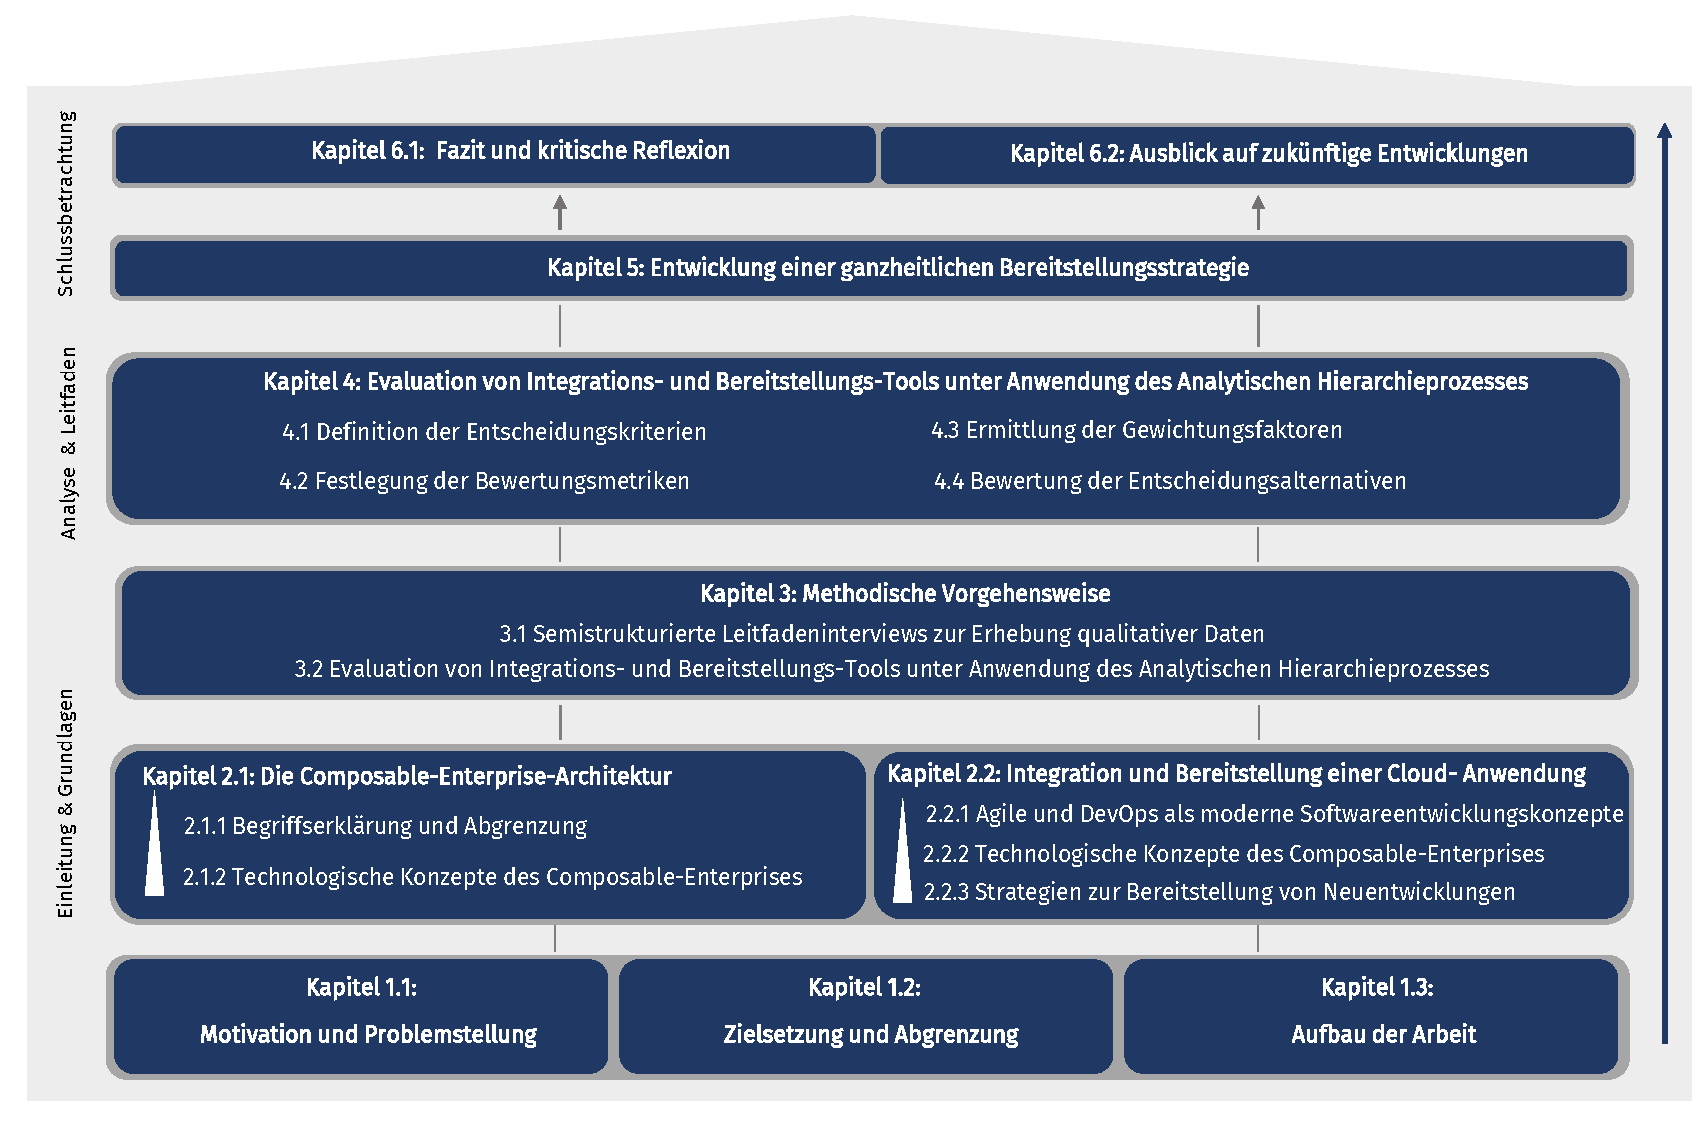
\includegraphics{Aufbau}}
		\caption[Aufbau der Arbeit]{Aufbau der Arbeit. Eigene Darstellung.}
		\label{fig:Aufbau}
	\end{figure}	
\end{center}
\vspace*{-15mm}
Im Methodikteil wird das gewählte Vorgehen zu den Experteninterviews, welche zur Erhebung qualitativer Daten durchgeführt werden, erläutert. Des Weiteren wird der \textit{Analytische Hierarchieprozesses} (\acs{AHP}), das Instrument zur Bestimmung des optimalen Bereitstellungs-Tools beschrieben. Im Teil der Durchführung erfolgt die Anwendung der Methodik auf die in den Experteninterviews erhobenen Daten. So werden im Rahmen des AHP-Verfahrens Entscheidungskriterien bestimmt, welche im Anschluss gewichtet und zur Bestimmung eines optimalen Bereitstellungs-Tools verwendet werden. In der folgenden Handlungsempfehlung wird eine ganzheitliche Bereitstellungsstrategie für CEA  entwickelt. Dabei wird das Ergebnis des AHP-Verfahrens analysiert und in Abhängigkeit verschiedener Unternehmensstrategien abgegrenzt. Abgerundet wird die Arbeit durch die Zusammenfassung der Erkenntnisse, einer kritischen Beleuchtung des Vorgehens und der Darstellung zukünftiger Ereignisse. 